%!TeX root = main.tex
%!encoding = UTF-8 Unicode

% \chapter{Platform for Combined Component- and System-Level EMC Measurements}
% \label{ch:TestBench}

\section{Measurement Environment}
The measurement platform aims to incorporate the discussed sensors into a classical power electronic application, while enabling the realization of the different measurement methoodologies for the the intrinsic EM emissions of the switching device.
Furthermore, a crosscheck with classical EMC measurements, namely a LISN measurement, is deployed in the measurement environment.

A picture of the measurement setup is shown in \fref{fig:pic_b2b_setup}.

%!TeX root = main.tex
%!encoding = UTF-8 Unicode

\section{Requirements for the Integrated EMC Measurement Environment}

The measurement platform must fulfill several requirements to enable reproducible and EMC-relevant characterization under realistic operating conditions.
First, it must provide a classical ground reference that represents the inverter chassis and allows physically meaningful coupling paths for high-frequency currents.
Second, the switching behavior of the test setup must be comparable to that of real applications, so that the measured emission spectra remain representative of practical converter operation.
Third, the platform must support the different measurement methodologies introduced in this work, in particular the operation of pulse chains with multiple consecutive switching events at a defined operating point.
Fourth, the setup must include a conducted-EMC reference measurement based on a LISN to allow direct comparison between intrinsic device emissions and standardized system-level quantities.
Fifth, additional noise sources introduced by the test environment must be minimized.
This includes filtering of the supply paths via the LISN, optical transmission of control signals, battery-powered gate-driver supplies, and a linear load implementation based on an air-core inductor.
Finally, the platform must allow stable operation during pulse-chain measurements without requiring active thermal management; therefore, passive cooling has to be sufficient for the intended operating regime.

The design choices discussed in the following section are derived directly from these requirements and are presented in the same logical order.

%!TeX root = main.tex
%!encoding = UTF-8 Unicode

\section{Design of the Measurement Environment}
The measurement setup implements the instrumentation required to satisfy the requirements defined in the previous section.
Its purpose is to capture the EMC-relevant high-frequency components of the three dominant intrinsic noise contributors: the drain-source voltages of the high-side and low-side devices and the commutation-loop current.
In parallel, a conventional conducted-EMC reference measurement via line impedance stabilization networks (LISNs) is integrated.

\begin{figure}[ht]
	\centering
	\import{./figures/6_Environment/}{"Diss_Pic_Setupv5.pdf_tex"}
	\caption{Photograph of measurement environment.}\label{fig:pic_b2b_setup}
\end{figure}

The setup is shown as a photograph in \fref{fig:pic_b2b_setup}, and its equivalent circuit is depicted in \fref{fig:ESB_b2b}.
The implementation follows the requirement order given above.

To realize a classical inverter-like ground reference, the primary half-bridge with the devices under test (DUTs), \mti{Q}{LS} and \mti{Q}{HS}, is mechanically coupled to an aluminum plate.
In this setup, the plate is primarily used as a defined, low-impedance return path for high-frequency ground currents toward the LISNs, thereby reproducing a physically meaningful chassis-like reference.

To ensure application-representative switching behavior, a conventional layout derived from an on-board charger is used.
This layout yields a commutation-loop inductance of \mi{L}{\sigma} = \SI{26}{nH}, which is comparatively high relative to state-of-the-art commutation loops based on purely coplanar designs.
However, the objective of this work is not to optimize the commutation loop itself, but to characterize the intrinsic emissions of the switching device under the given parasitic conditions.

To enable pulse-chain operation for thermal-noise reduction, a back-to-back converter topology is employed, in which both half-bridges share a common DC link and are separated by the main filters of the LISNs.
This architecture allows repeated switching events to be generated at nearly identical operating conditions, thereby improving repeatability and increasing the statistical robustness of the derived frequency-domain spectra.

\begin{figure}[ht]
	\centering
	\import{./figures/6_Environment/}{"Diss_ESB_B2B.pdf_tex"}
	\caption{Equivalent circuit diagram of the back-to-back converter measurement setup.}\label{fig:ESB_b2b}
\end{figure}



To include a standardized conducted-EMC reference, both converter sides are connected via LISNs.
This enables direct comparison between intrinsic terminal quantities and system-level conducted-noise metrics.
Since the focus of this dissertation is the direct characterization of intrinsic emissions, the detailed interaction between the \mi{v}{DS} measurement and the LISN result is not discussed here; an in-depth analysis is provided in~\cite{kragl_impact_2024}.

% For this paper only the raw emissions are considered and hence, no LISNs measurements are shown.
% For an analysis of the correlation between raw emissions and system-level LISN measurement, please refer to~\cite{kragl_impact_2024}.

To suppress additional noise introduced by the environment, the secondary half-bridge is intentionally designed as a low-disturbance auxiliary stage.
It consists of \mti{Q}{LS,aux} and \mti{Q}{HS,aux}, with devices rated at twice the current of the DUTs and operated at five times the gate resistance.
This reduces the switching speed and therefore the high-frequency spectral contribution of the auxiliary branch.
In addition, the auxiliary devices are placed adjacent to, but not directly on, the aluminum plate to avoid an unintended direct coupling path into the measurement ground.

Further mitigation measures follow directly from the requirements: high-frequency isolation between the two half-bridges is established through the LISN main filters, digital control signals are transmitted via optical links, and the gate-driver supplies are battery powered.
Moreover, the load path is implemented as a linear air-core inductor to avoid nonlinear magnetic behavior that could distort the measured spectral content.

Finally, thermal operation is constrained to a regime in which passive cooling remains sufficient during pulse-chain measurements.



\chapter{Methodological Validation and Quantification of Electromagnetic Emissions}

Having realized the methodology of Chapter~\ref{ch:Methods} through the instrumentation and platform of the preceding chapter, this chapter validates the resulting measurement environment on real switching events before it is applied to the parameter studies of the next chapter.
First, the impact of the individual noise-reduction steps, oversampling and averaging, high-pass compensation, and the TDF, is demonstrated on a measured spectrum.
The intrinsic emission measurements are then cross-referenced against a classical system-level LISN measurement to confirm their consistency with established EMC practice.
Finally, the switching-event-resolved frequency-domain analysis is demonstrated, isolating the spectral contribution of the active-on, active-off, passive-on, and passive-off switching events.

%!TeX root = main.tex
%!encoding = UTF-8 Unicode

\section{Demonstration of Noise-Reduction Steps}
First, the influence of the individual noise-reduction steps on high-frequency drain-source-voltage measurements is demonstrated.

\begin{figure}[ht]
	\centering
	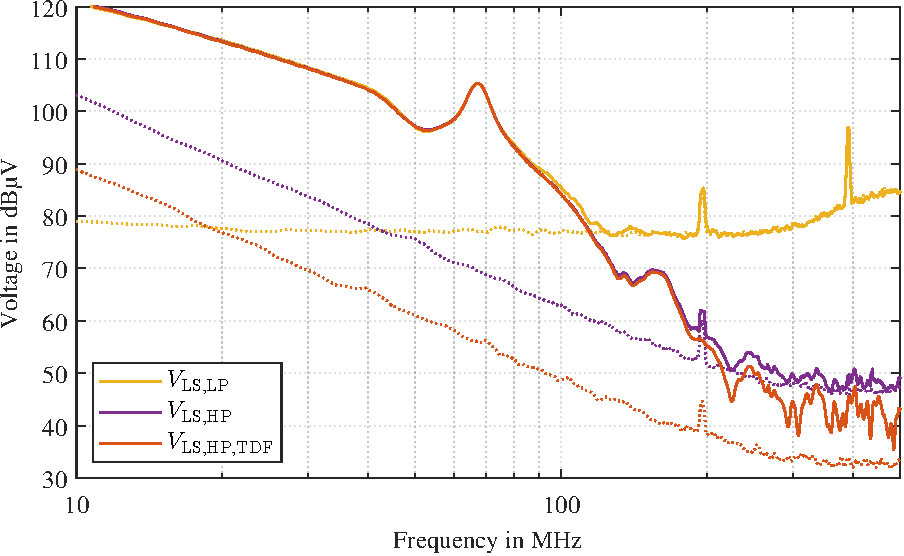
\includegraphics[scale = 1]{figures/7_MeasurementResults/MR_Methodology.pdf}
	\caption{Impact of different noise-reduction steps on the measurement (solid line) and the corresponding noise floor (dotted line).}\label{fig:MR_Methodology}
\end{figure}

Figure~\ref{fig:MR_Methodology} shows the spectrum used later, measured at the active low-side switch of an SiC MOSFET with an active area of \SI{5}{mm^2}, for the low-pass, high-pass, and TDF signals.
For each signal, two measurements are performed: one with DUT operation (signal of interest) and one background measurement without DUT operation to determine the noise floor, which is shown as a dotted line.
To evaluate both quantities in the same spectrum plot, the measured signals are compensated using the transfer functions in \eref{eq:HP_comp} and \eref{eq:TF_Shunt}.



In the low-pass spectrum, which corresponds to conventional measurements, the noise floor is around \SI{76}{dB\micro\volt}, which is sufficient for analyzing the switching transient up to \SI{115}{MHz}.
For higher frequencies, the signal falls below the noise level, which is why the high-pass measurement is necessary.

The high-pass measurement remains above the noise floor up to \SI{220}{MHz}, which is a significant improvement over the low-pass path.
However, the signal still decreases faster over frequency than the noise floor, so the SNR decreases at higher frequencies.
In the high-pass background measurement, the compensated noise floor decreases with frequency because the approximately constant noise measurement is divided by the increasing high-pass gain.

In a final step, the TDF filter is applied in post-processing, further reducing the noise floor by about \SI{15}{dB}.
This enables analysis of the switching transient up to \SI{500}{MHz}.





% \section{Demonstration of Switching Event Resolved Frequency Domain Analysis}
% In this section the switching event resolved frequency domain analysis is demonstrated, which provides a more detailed analysis of the noise contribution of the different switching events.
% The methodology is explained in detail in Section~\ref{subsec:SpectralSeparation}.
% The test results are for a first generation, Robert Bosch SiC MOSFET operated at $\mi{V}{DC} = \SI{800}{V}$, $\mi{I}{load} = \SI{60}{A} = \mi{I}{N,MOSFET}$, and $\mi{R}{G} = \SI{5.6}{\Omega}$, with a commutation-loop inductance of $\mi{L}{\sigma} = \SI{24}{nH}$ and an ambient temperature of $T = \SI{30}{\celsius}$.

% Figure~\ref{fig:MR_Demo_SpekSep_TD} shows the time-domain measurement results of the demonstration of switching event resolved frequency domain analysis.
% The two measured voltages of the active and passive switch are separated into the four artificial signals of the active-on, active-off, passive-on, and passive-off switching events.



% \begin{figure}[ht]
% 	\centering
% 	\begin{subfigure}[t]{\textwidth}
% 		\centering
% 		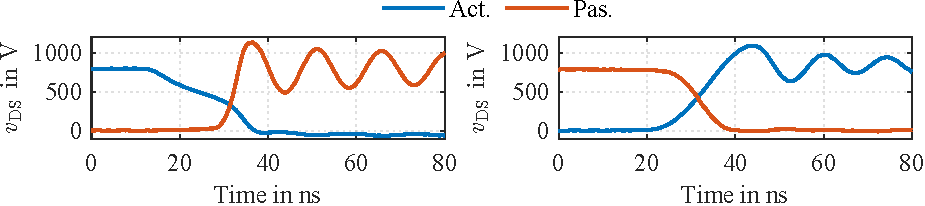
\includegraphics[scale = 1]{figures/6_Environment/MR_Demo_SpekSep/MR_Demo_SpekSep_ActPasVoltage_TD.pdf}
% 		\subcaption{Time-domain voltage measurement results of the active and passive switches.}
% 		\label{fig:MR_L_constE_Sweep_Voltage_TD}
% 	\end{subfigure} 
    
% 	\vspace{0.5cm}	
	
% 	\begin{subfigure}[t]{\textwidth}
% 		\centering
% 		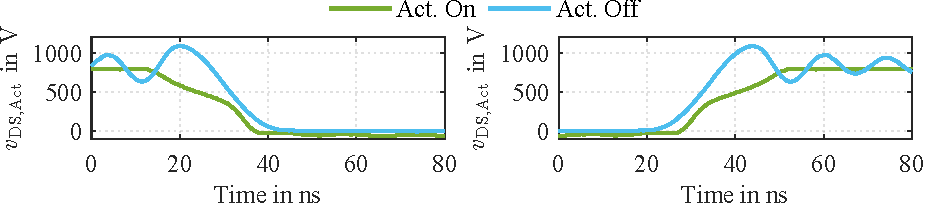
\includegraphics[scale = 1]{figures/6_Environment/MR_Demo_SpekSep/MR_Demo_SpekSep_ActVoltage_TD.pdf}
% 		\subcaption{Separated, artificial switching events of the active switch.}
% 		\label{fig:MR_L_constE_Sweep_ActVoltage_TD}
% 	\end{subfigure} 

% 	\vspace{0.5cm}

% 	\begin{subfigure}[t]{\textwidth}
% 		\centering
% 		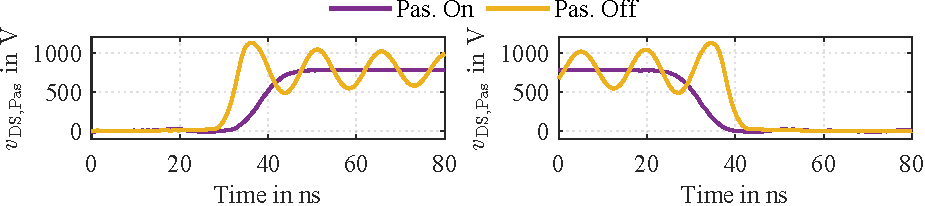
\includegraphics[scale = 1]{figures/6_Environment/MR_Demo_SpekSep/MR_Demo_SpekSep_PasVoltage_TD.pdf}
% 		\subcaption{Separated, artificial switching events of the passive switch.}
% 		\label{fig:MR_L_constE_Sweep_PasVoltage_TD}
% 	\end{subfigure} 

% 	\caption{Time-domain results of the demonstration of switching event resolved frequency domain analysis.}
% 	\label{fig:MR_Demo_SpekSep_TD}
% \end{figure}


% These measurements show the typical behavior of a MOSFET switched with a constant gate resistance at room temperature. 
% The observations can be summarized as follows:
% \begin{enumerate}
% 	\item The passive-off event exhibits a higher overvoltage than the active-off event (\SI{1130}{V} compared with \SI{1080}{V}), and this overvoltage increases with temperature because the body diode stores more bipolar charge.
% 	\item The passive-off event responds purely passively to the excitation transient, whereas the active-off event initially shows an approximately linear voltage increase controlled by the gate driver. This is followed by an inductive overshoot, only after which the output capacitance and the commutation-cell inductance begin to oscillate passively.
% 	\item The on-events also behave differently: the active-on event initially exhibits a voltage drop caused by the inductive voltage drop across the commutation-cell inductance, followed by the actual voltage commutation controlled by the gate driver. This creates two distinct transient times, and the faster or larger one dominates the spectrum.
% 	\item In contrast, the passive-on event shows a smooth voltage transient, which is the reaction of the passive $LC$ tank to the controlled active-off transient and is therefore smoothed by the impedance of the tank.
% \end{enumerate}

% These time-domain observations provide the physical basis for the event-resolved interpretation of the frequency-domain spectra. To understand the impact of the four distinct switching events on the measured spectrum, the same snap-and-mirror method is applied to the corresponding high-pass measurements and combined with the TDF filter in post-processing. The resulting frequency-domain results are shown in \fref{fig:MR_Demo_SpekSep_FD}.
% The general functionality of the snap-and-mirror method is demonstrated by the observation that, for both the active and passive switch emission spectra, one of the two contributing switching events (on or off) dominates specific frequency ranges, while the other contributes only marginally.

% \begin{figure}[!t]
% 	\centering
% 	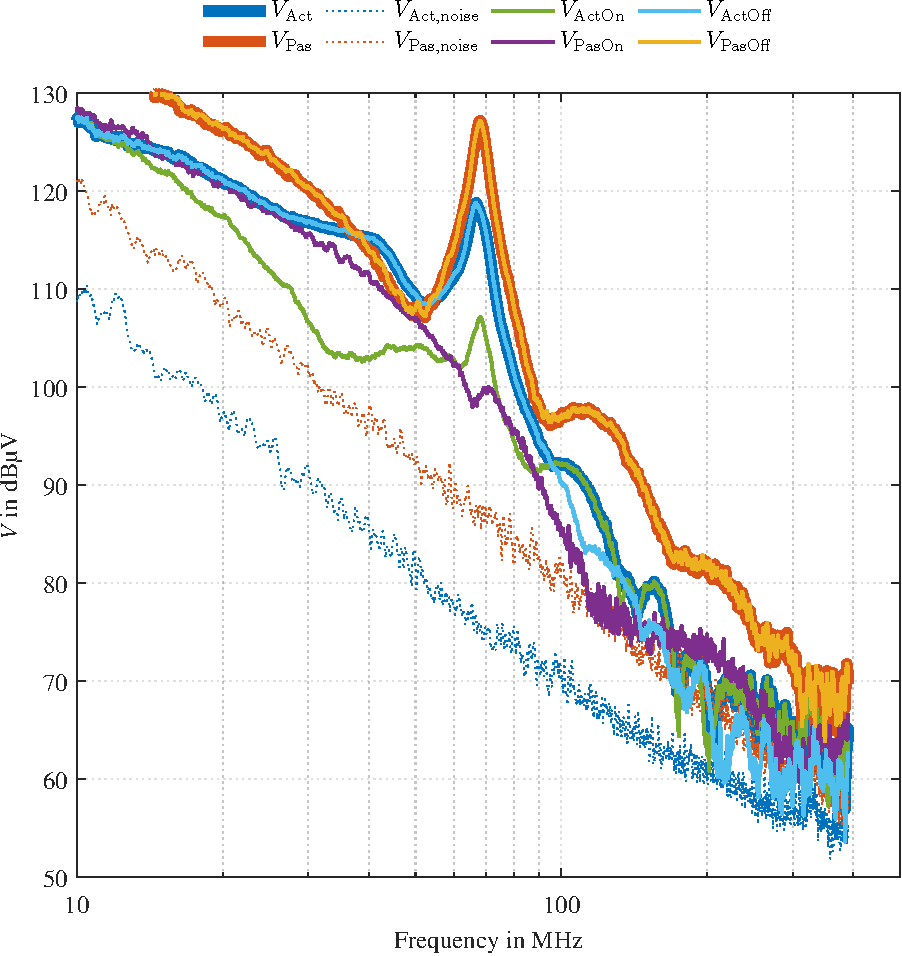
\includegraphics[scale = 1]{figures/6_Environment/MR_Demo_SpekSep/MR_Demo_SpekSep_FD.pdf}
% 	\caption{Frequency-domain measurement results of the demonstration of switching event resolved frequency domain analysis.}\label{fig:MR_Demo_SpekSep_FD}
% \end{figure}

% In addition, several consistent trends can be identified in the frequency-domain results over a wide range of operating conditions. These are summarized as follows:
% \begin{enumerate}
% 	\item The passive switch, and in particular the passive-off event, exhibits consistently higher emission than the active switch. This trend is consistent with the general EMC experience in the laboratory and is attributed to the larger overvoltage and stronger ringing of the passive switch.
% 	\item For the active switch, the turn-off event dominates the lower-frequency range and the resonance region; however, above approximately \SI{100}{MHz}, the turn-on event becomes dominant and reaches up to \SI{8}{dB} higher emission. The exact crossover frequency depends on the switching speed.
% 	\item A slight mismatch between the resonance frequencies of the active and passive switch is observed (\SI{66}{MHz} compared with \SI{69}{MHz}). 
% 	This difference increases for smaller chip sizes and lower capacitances, as predicted by the coupling model in \cite{liu_modeling_2016}. 
% 	The underlying cause is the different coupling of the oscillation into the gate loop of the active switch and the passive switch, respectively.
% 	\item A small resonance is observed in the active-on event, which is attributed to imperfect shielding and capacitive coupling from the passive-off event into the active-on contribution. 
% 	This effect is not observed in the passive-on event because the active-off event is significantly smaller in amplitude and therefore couples less strongly.
% 	\item Although the passive-on transient is faster than the active-on transient, its emission is lower in the high-frequency range. 
% 	This is due to the second, faster transient of the active-on event, which is steeper than the initial inductive voltage drop and therefore contributes more strongly to the high-frequency spectrum.
% 	\item The noise floor of the passive switch is higher than that of the active switch. 
% 	This is a consequence of the larger signal amplitude and the associated requirement for a larger vertical scale on the oscilloscope, which increases the measurement noise floor.
% \end{enumerate}

% Overall, the event-resolved analysis provides a detailed and physically transparent decomposition of the total noise emission into its dominant switching-event contributors. 
% This new method enables a much more precise assessment of the individual mechanisms that shape the measured spectrum and reveals which transient events actually limit the EMC performance at a given frequency range. In practical terms, this allows for targeted EMC debugging, since only the noisiest contributor determines the emission limit in a given frequency band. 
% As a result, optimization can be focused on the dominant source rather than on the total waveform, enabling faster or more aggressive switching of other contributors without increasing the total emitted noise. 
% This is particularly valuable for balancing switching losses and EMC performance, because the design space can be explored more deliberately when the limiting mechanism is known and not obscured by the aggregate signal.


%!TeX root = main.tex
%!encoding = UTF-8 Unicode

\section{LISN Measurement for System-Level Cross Reference}

This section presents the LISN measurements as a cross-reference to the intrinsic emission measurements.
As an example, a \SI{1200}{V} SiC MOSFET in a D2PAK package is used as the DUT, and the standard gate-resistance variation test is performed.
Since the oscilloscope ground is fixed to the aluminum base plate, no current measurement is carried out in this configuration.
The measurement results are shown in \fref{fig:MR_LISN_Voltage_TD} and \fref{fig:MR_LISN_LISN_TD} for the time domain and in \fref{fig:MR_LISN_FD} for the frequency domain.

\begin{figure}[ht]
	\centering
	\tikzsetnextfilename{MR_LISN_Voltage_TD}
	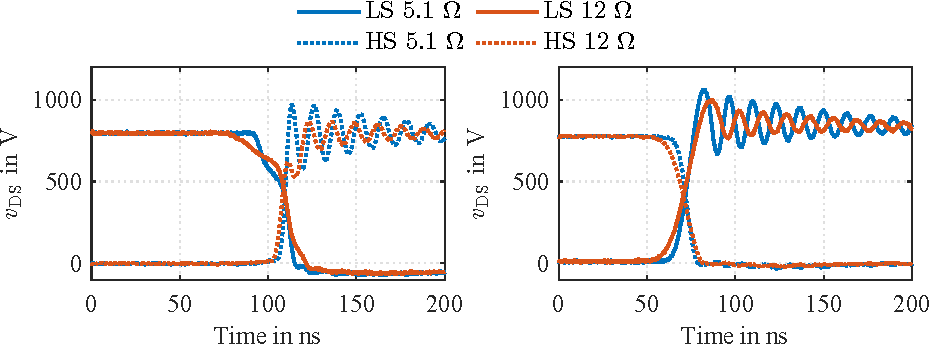
\includegraphics[scale=1]{figures/6_Environment/MR_LISN/MR_LISN_Voltage_TD.pdf}
	\caption{Time-domain measurement of low-side and high-side voltages for two gate resistances at \SI{800}{V} and \SI{60}{A} for PMTX03.}\label{fig:MR_LISN_Voltage_TD}
\end{figure}

\begin{figure}[ht]
	\centering
	\tikzsetnextfilename{MR_LISN_LISN_TD}
	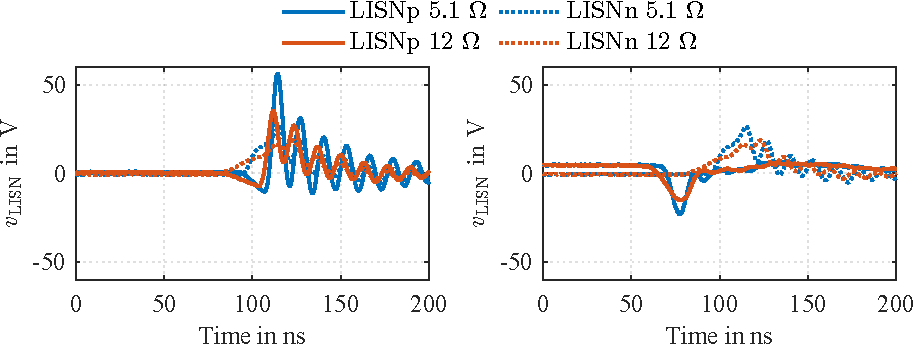
\includegraphics[scale=1]{figures/6_Environment/MR_LISN/MR_LISN_LISN_TD.pdf}
	\caption{Time-domain measurement of LISN voltages for two gate resistances at \SI{800}{V} and \SI{60}{A} for PMTX03.}\label{fig:MR_LISN_LISN_TD}
\end{figure}

The time-domain plots confirm the expected influence of increased gate resistance: the switching speed decreases and the voltage transitions become slower.
This is the classical behavior observed in gate-resistance variation studies.
In contrast, the frequency-domain plots provide more relevant information for EMC analysis, because they reveal how system-level parasitics and return paths shape the emission behavior.
These LISN measurements represent the state of the art for semiconductor-oriented EMC analysis, and their limitations are discussed in the following.

The upper graph of \fref{fig:MR_LISN_FD} shows the intrinsic emissions measured with the high-pass output of the DAVP.
The lower two graphs show the conventional LISN voltages, first directly and then in the translated common-mode and differential-mode components.
The corresponding voltages can be calculated as
\begin{equation}
    \mi{v}{CM} = \frac{1}{2}\cdot(\mi{v}{LISNp} + \mi{v}{LISNn})
\end{equation}

\begin{equation}
    \mi{v}{DM} = \frac{1}{2}\cdot(\mi{v}{LISNp} - \mi{v}{LISNn})
\end{equation}

When the LISN voltages are examined, the onset of the noise floor becomes evident slightly above the resonance frequency at \SI{75}{MHz}.
This noise floor is the same as the one introduced in Sec.~\ref{sec:methods} and is only marginally lower than that of a direct drain-source voltage measurement, because the switching node couples capacitively to the cooler and then to the LISN terminals.
However, this creates a first-order transfer function, while the actual signal falls with second-order or even higher-order behavior.
This is clearly visible in the high-pass measurement of the drain-source voltages, which span a much wider range from \SI{40}{dB\mu V} to \SI{140}{dB\mu V}, compared to only about \SI{30}{dB} for the LISN voltages.
Consequently, the maximum measurable frequency in the system-level measurement with the LISN is approximately \SI{150}{MHz}, while the DAVP measures up to \SI{400}{MHz}.

\begin{figure}[ht]
	\centering
	\tikzsetnextfilename{MR_LISN_FD}
	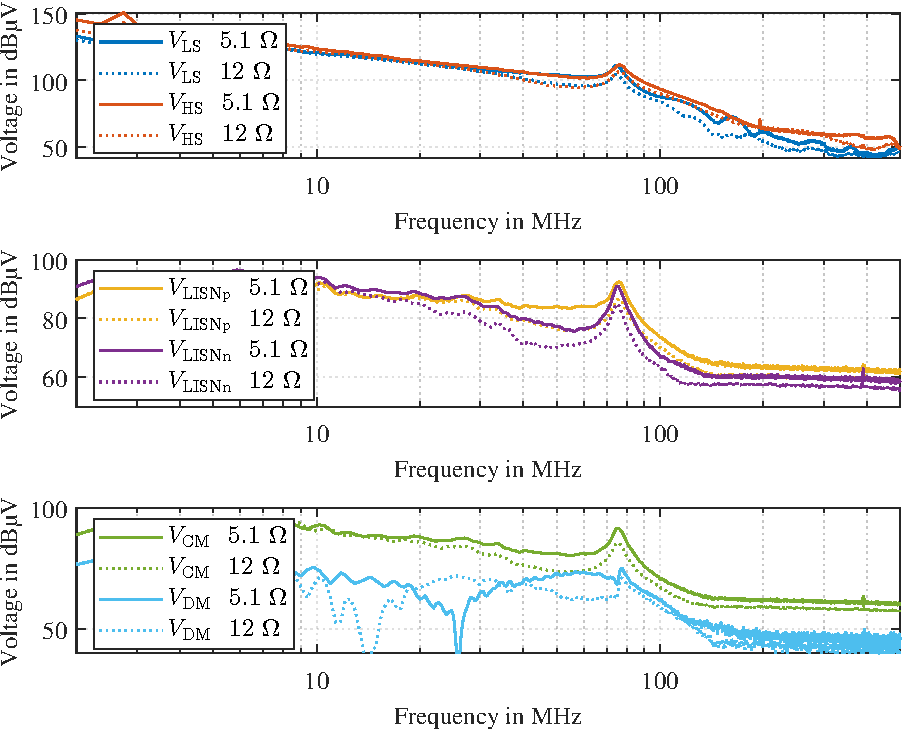
\includegraphics[scale=1]{figures/6_Environment/MR_LISN/MR_LISN_FD.pdf}
	\caption{Frequency-domain measurement of drain-source and LISN voltages for two gate resistances at \SI{800}{V} and \SI{60}{A} for PMTX03.}\label{fig:MR_LISN_FD}
\end{figure}

Nevertheless, some additional insight can be gained from the data.
When the high-side and low-side main resonances are compared, a small mismatch in resonance frequency becomes visible.
This is caused by passive turn-off, where the oscillation couples into the gate and the corresponding capacitances create a slight mismatch.
This effect does not occur during active turn-off, because the gate driver holds the gate capacitance constant.
This behavior is discussed in detail in \cite{paper}.
A similar mismatch can also be observed in the LISN voltages.
While the peak of \mi{v}{LISNp} occurs at \SI{76}{MHz}, the peak of \mi{v}{LISNn} occurs at \SI{74}{MHz}, which corresponds exactly to the resonances of \mi{v}{DS,HS} and \mi{v}{DS,LS}, respectively.
This can be explained by the positioning of the high-side and low-side MOSFETs relative to the positive and negative LISN terminals.
From \fref{fig:pic_b2b_setup}, it is evident that the high-side switch \mi{Q}{HS} is placed closer to LISNp, while \mi{Q}{LS} is placed closer to LISNn.
The respective noise of each switch therefore follows the lowest-impedance or shortest return path.
Furthermore, the general slope of the raw emission \mi{v}{DS} is also visible in the system-level measurements \mi{v}{LISN}, confirming the validity of the complete measurement approach.

In future work, the transfer function between these two measurement types should be investigated.
This would enable system-level information to be extracted from raw emission measurements and extend the usable range of this approach.






%!TeX root = main.tex
%!encoding = UTF-8 Unicode

\section{Demonstration of Switching Event Resolved Frequency Domain Analysis}
In this section the switching event resolved frequency domain analysis is demonstrated, which provides a more detailed analysis of the noise contribution of the different switching events.
The methodology is explained in detail in Section~\ref{subsec:SpectralSeparation}.
The test results are for a first generation, Robert Bosch SiC MOSFET operated at $\mi{V}{DC} = \SI{800}{V}$, $\mi{I}{load} = \SI{60}{A} = \mi{I}{N,MOSFET}$, and $\mi{R}{G} = \SI{5.6}{\Omega}$, with a commutation-loop inductance of $\mi{L}{\sigma} = \SI{24}{nH}$ and an ambient temperature of $T = \SI{30}{\celsius}$.

Figure~\ref{fig:MR_Demo_SpekSep_TD} shows the time-domain measurement results of the demonstration of switching event resolved frequency domain analysis.
The two measured voltages of the active and passive switch are separated into the four artificial signals of the active-on, active-off, passive-on, and passive-off switching events.



\begin{figure}[ht]
	\centering
	\begin{subfigure}[t]{\textwidth}
		\centering
		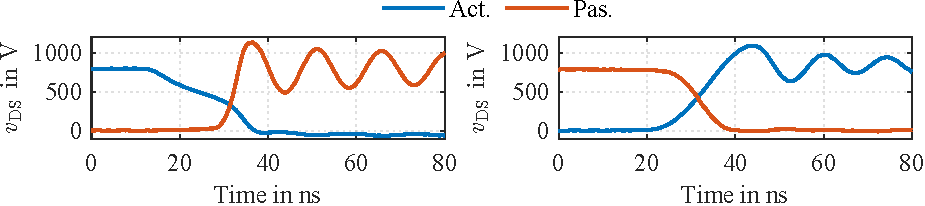
\includegraphics[scale = 1]{figures/6_Environment/MR_Demo_SpekSep/MR_Demo_SpekSep_ActPasVoltage_TD.pdf}
		\subcaption{Time-domain voltage measurement results of the active and passive switches.}
		\label{fig:MR_L_constE_Sweep_Voltage_TD}
	\end{subfigure} 
    
	\vspace{0.5cm}	
	
	\begin{subfigure}[t]{\textwidth}
		\centering
		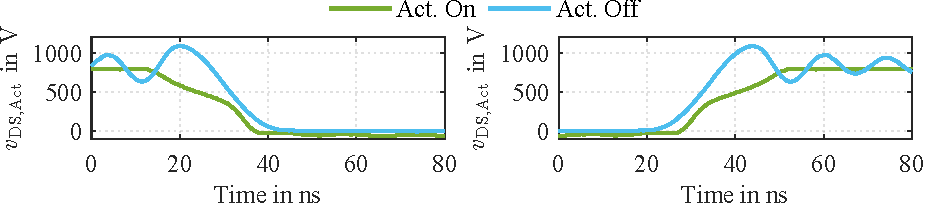
\includegraphics[scale = 1]{figures/6_Environment/MR_Demo_SpekSep/MR_Demo_SpekSep_ActVoltage_TD.pdf}
		\subcaption{Separated, artificial switching events of the active switch.}
		\label{fig:MR_L_constE_Sweep_ActVoltage_TD}
	\end{subfigure} 

	\vspace{0.5cm}

	\begin{subfigure}[t]{\textwidth}
		\centering
		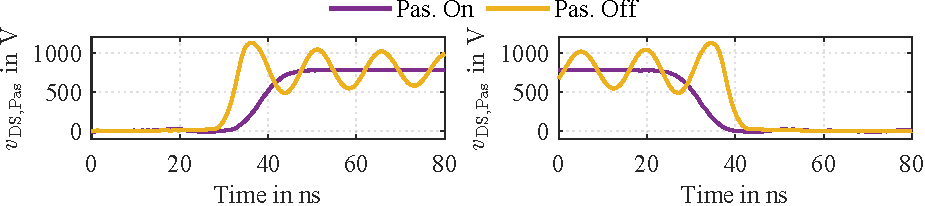
\includegraphics[scale = 1]{figures/6_Environment/MR_Demo_SpekSep/MR_Demo_SpekSep_PasVoltage_TD.pdf}
		\subcaption{Separated, artificial switching events of the passive switch.}
		\label{fig:MR_L_constE_Sweep_PasVoltage_TD}
	\end{subfigure} 

	\caption{Time-domain results of the demonstration of switching event resolved frequency domain analysis.}
	\label{fig:MR_Demo_SpekSep_TD}
\end{figure}


These measurements show the typical behavior of a MOSFET switched with a constant gate resistance at room temperature. 
The observations can be summarized as follows:
\begin{enumerate}
	\item The passive-off event exhibits a higher overvoltage than the active-off event (\SI{1130}{V} compared with \SI{1080}{V}), and this overvoltage increases with temperature because the body diode stores more bipolar charge.
	\item The passive-off event responds purely passively to the excitation transient, whereas the active-off event initially shows an approximately linear voltage increase controlled by the gate driver. This is followed by an inductive overshoot, only after which the output capacitance and the commutation-cell inductance begin to oscillate passively.
	\item The on-events also behave differently: the active-on event initially exhibits a voltage drop caused by the inductive voltage drop across the commutation-cell inductance, followed by the actual voltage commutation controlled by the gate driver. This creates two distinct transient times, and the faster or larger one dominates the spectrum.
	\item In contrast, the passive-on event shows a smooth voltage transient, which is the reaction of the passive $LC$ tank to the controlled active-off transient and is therefore smoothed by the impedance of the tank.
\end{enumerate}

These time-domain observations provide the physical basis for the event-resolved interpretation of the frequency-domain spectra. To understand the impact of the four distinct switching events on the measured spectrum, the same snap-and-mirror method is applied to the corresponding high-pass measurements and combined with the TDF filter in post-processing. The resulting frequency-domain results are shown in \fref{fig:MR_Demo_SpekSep_FD}.
The general functionality of the snap-and-mirror method is demonstrated by the observation that, for both the active and passive switch emission spectra, one of the two contributing switching events (on or off) dominates specific frequency ranges, while the other contributes only marginally.

\begin{figure}[!t]
	\centering
	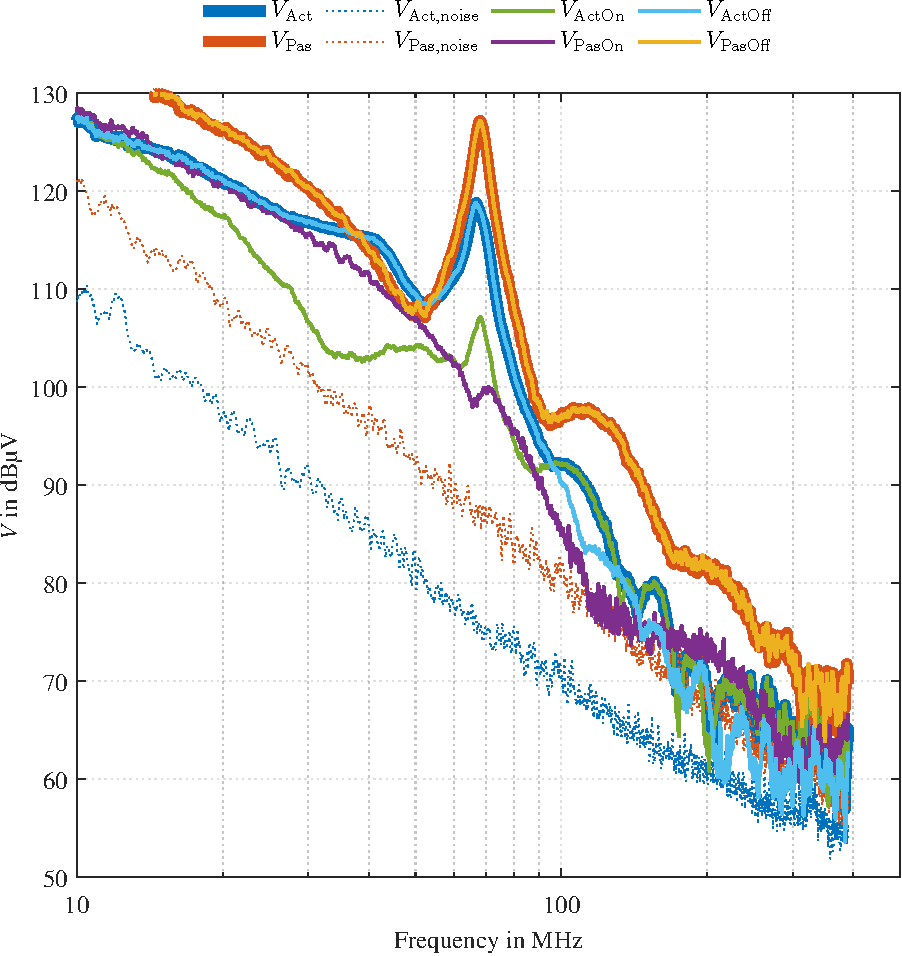
\includegraphics[scale = 1]{figures/6_Environment/MR_Demo_SpekSep/MR_Demo_SpekSep_FD.pdf}
	\caption{Frequency-domain measurement results of the demonstration of switching event resolved frequency domain analysis.}\label{fig:MR_Demo_SpekSep_FD}
\end{figure}

In addition, several consistent trends can be identified in the frequency-domain results over a wide range of operating conditions. These are summarized as follows:
\begin{enumerate}
	\item The passive switch, and in particular the passive-off event, exhibits consistently higher emission than the active switch. This trend is consistent with the general EMC experience in the laboratory and is attributed to the larger overvoltage and stronger ringing of the passive switch.
	\item For the active switch, the turn-off event dominates the lower-frequency range and the resonance region; however, above approximately \SI{100}{MHz}, the turn-on event becomes dominant and reaches up to \SI{8}{dB} higher emission. The exact crossover frequency depends on the switching speed.
	\item A slight mismatch between the resonance frequencies of the active and passive switch is observed (\SI{66}{MHz} compared with \SI{69}{MHz}). 
	This difference increases for smaller chip sizes and lower capacitances, as predicted by the coupling model in \cite{liu_modeling_2016}. 
	The underlying cause is the different coupling of the oscillation into the gate loop of the active switch and the passive switch, respectively.
	\item A small resonance is observed in the active-on event, which is attributed to imperfect shielding and capacitive coupling from the passive-off event into the active-on contribution. 
	This effect is not observed in the passive-on event because the active-off event is significantly smaller in amplitude and therefore couples less strongly.
	\item Although the passive-on transient is faster than the active-on transient, its emission is lower in the high-frequency range. 
	This is due to the second, faster transient of the active-on event, which is steeper than the initial inductive voltage drop and therefore contributes more strongly to the high-frequency spectrum.
	\item The noise floor of the passive switch is higher than that of the active switch. 
	This is a consequence of the larger signal amplitude and the associated requirement for a larger vertical scale on the oscilloscope, which increases the measurement noise floor.
\end{enumerate}

Overall, the event-resolved analysis provides a detailed and physically transparent decomposition of the total noise emission into its dominant switching-event contributors. 
This new method enables a much more precise assessment of the individual mechanisms that shape the measured spectrum and reveals which transient events actually limit the EMC performance at a given frequency range. In practical terms, this allows for targeted EMC debugging, since only the noisiest contributor determines the emission limit in a given frequency band. 
As a result, optimization can be focused on the dominant source rather than on the total waveform, enabling faster or more aggressive switching of other contributors without increasing the total emitted noise. 
This is particularly valuable for balancing switching losses and EMC performance, because the design space can be explored more deliberately when the limiting mechanism is known and not obscured by the aggregate signal.




